%%%%%%%%%%%%%%%%%%%%%%%%%%%%%%% Inciso 01A:
$a$) \begin{lstlisting}
  {with {a { + 2 2 } }
    {with {b { + a a } }
      {with {foo { fun {x} {- x b } } }
        {with {a {- 2 2 } }
          {with {b {- a a } }
            {foo -3 } } } } }
\end{lstlisting} 

Primero construyamos las pilas de ambientes, con
respecto al régimen de evaluación, esto es

\begin{multicols}{2}    
  % Régimen Perezoso
  $*$) Con evaluación perzosa:
  \begin{center}
    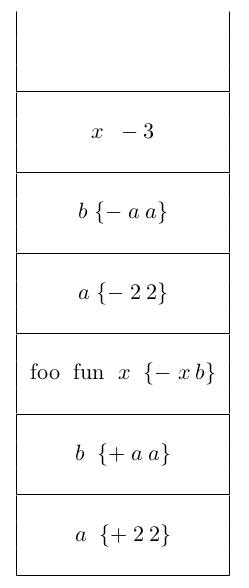
\includegraphics[scale=0.40]{./Perezosa}
  \end{center}
  
  \begin{enumerate}
  \item Evaluación perezosa y alcance estático.
  \item Evaluación perezosa y alcance dinámico.
  \end{enumerate}
  
  % Régimen Glotón
  $*$) Con evaluación glotona:
  \begin{center}
    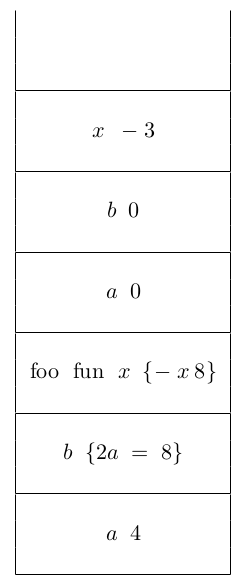
\includegraphics[scale=0.40]{./Glotona}
  \end{center}

  \begin{enumerate}
  \item Evaluación glotona y alcance estático.
  \item Evaluación glotona y alcance dinámico.
  \end{enumerate}

\end{multicols}


